\documentclass[a4paper]{article}
\setlength{\parskip}{\baselineskip}
\let\oldbibliography\thebibliography
\renewcommand{\thebibliography}[1]{%
  \oldbibliography{#1}%
  \setlength{\itemsep}{0pt}%
}

% First load extension packages
\usepackage[a4paper,margin=25mm]{geometry}    % page layout
\usepackage{setspace} \onehalfspacing         % line spacing
\usepackage{amsfonts,amssymb,amsmath}         % useful math extensions
\usepackage{graphicx}                         % graphics import
\graphicspath{{../figs/}}
\pdfpageattr{/Group << /S /Transparency /I true /CS /DeviceRGB>>}
\usepackage[colorlinks=true, allcolors=black]{hyperref}
\usepackage{hhline}
\usepackage{subcaption}
% Change paragraph indentation
\setlength{\parskip}{10pt}
\setlength{\parindent}{0pt}
\usepackage[toc]{multitoc}
%\renewcommand*{\multicolumntoc}{2}
\setlength{\columnsep}{36pt}
% User-defined commands
\newcommand\numberthis{\addtocounter{equation}{1}\tag{\theequation}}
% topmatter
\title{\vspace{-50pt}\huge\bfseries Developing a Coarse-Grained Climate Model
to Investigate Long-Term Behaviour}

\author{Liam Wheen \\ Supervised by Dr O.\ Benjamin}

\date{\today}
\pagenumbering{gobble}
% main body
\begin{document}
\begin{titlepage}
\maketitle
\hrule
\vspace{-10pt}
\begin{abstract}
\noindent
This is the abstract.
\end{abstract}
\hrule
\end{titlepage}
%\vspace{20pt}
\newpage
\pagenumbering{gobble}
%\begin{spacing}{0.6}
\tableofcontents
%\end{spacing}
\newpage
\pagenumbering{arabic}
\section{Introduction}
\section{Budyko Model}
The Budyko model is an energy balance model (EBM) that explores the positive
feedback effect of polar ice cap albedo. The increased reflectivity of polar
ice caps causes Earth to receive less net energy from the sun across these
regions. If a sufficient amount of Earth's surface is covered in ice, 
global temperatures drop and the polar ice caps advance towards the equator.
Conversely, if the ice caps only exist at very high latitudes, then the reduced
reflectivity will cause Earth's temperature to rise, and this ice-line to
recede further.

A number of assumptions are made in order for this EBM to work. Temperature
is modelled as varying only across latitude, reducing the domain of the
system from a spherical surface, to a 1-dimensional temperature profile. In
order to simplify integral that span the latitudes, the
domain is described using $y = \sin(\varphi)$, where $\varphi$ is latitude.
To simplify the system further, the Earth is treated as an entirely water-based
planet. This allows for the differences in ground reflectivity to be ignored,
focusing only on the albedo of water, and ice. The Earth is also modelled as
symmetric across the equator, allowing for only one half of the domain to be
considered, i.e. $y\in [0,1]$. The impact of this last assumption is
investigated in section ----add ref----.

The dynamical equation for temperature consists of three components. They
describe the flow of energy into, out of, and around Earth.
The first of these is incoming solar radiation, insolation.
This depends on the irradiance given out by the sun, as well as the distance
and orientation of the Earth to the sun. The amount of insolation experienced
at different latitudes varies proportional to the
cosine of the angle between the ecliptic plane and the corresponding point on
Earth. This is why the poles receive less insolation over the year than the
equator.

The next component is the outgoing infra-red radiation.
This is approximated to linearly depend on the temperature of Earth. Although
the energy flow occurring within Earth's atmosphere is far more complex, 
empirical data was used to establish the net flow of heat from
Earth to the first order.

The final component of energy flow is the transport of energy around Earth, from
the hot equator to the relatively cooler poles. This depends on the difference
between the average temperature of the earth and the temperature at each
latitude.

Combining these elements gives the dynamical equation for temperature to be

\[
  R\frac{\partial T(y,t)}{\partial t} = \underbrace{Qs(y) (1-\alpha(y,\eta))}_{\text{Insolation}}
  - \underbrace{(A+BT(y,t))}_{\text{Reradiation}}
  + \underbrace{C(\bar{T}-T(y,t))}_{\text{Transport}},
\]

where $A, B, C,$ and $R$ are constants found using empirical data, $Q$ is the
annually averaged solar insolation experienced across the Earth, distributed
according to latitude with the function 

\[
  s(y) = 1+ \frac{1}{2}c_\beta(3y^2-1) 
\]

where $c_\beta = \frac{5}{16}(3\sin^2\beta - 2)$ and $\beta$ is Earth's axial
tilt or obliquity.


\begin{figure}
\centering
\begin{subfigure}{.5\textwidth}
  \centering
  \includegraphics[width=\linewidth]{demo_budyko_0.pdf}
  \caption{0 Years}
\end{subfigure}%
\begin{subfigure}{.5\textwidth}
  \centering
  \includegraphics[width=\linewidth]{demo_budyko_1.pdf}
  \caption{10 Years}
\end{subfigure}
\begin{subfigure}{.5\textwidth}
  \centering
  \includegraphics[width=\linewidth]{demo_budyko_2.pdf}
  \caption{3000 Years}
\end{subfigure}%
\begin{subfigure}{.5\textwidth}
  \centering
  \includegraphics[width=\linewidth]{demo_budyko_3.pdf}
  \caption{10\,000 Years}
\end{subfigure}
\caption{Snapshots of a Budyko simulation starting with 0$^\circ$C at all
latitudes and the ice line at $y=0.5$. The orbital parameters used are shown in
Table \ref{tab:orbital_params}. We first see the temperature profile
equilibrate within 10 years. The ice line then recedes 
towards the stable equilibrium point at $y=0.9544$, taking 10\,000 years to get
within 3\% of this point.}
\label{fig:budyko_demo}
\end{figure}


\section{Insolation}
To implement an asymmetrical version of the Budyko model, the difference
between the northern and southern hemispheres must first be established.
Insolation is solar irradiance integrated over time, however we are usually
interested in the average insolation over a given time period, hence the units
for both irradiance and average insolation are W\,m$^{-2}$. Insolation will first
be modelled on a daily basis to see how insolation varies throughout a year at
different latitudes, then on a yearly basis. All simulations that depend on the
Milankovitch cycles take this data from Laskar \cite{milanko_data}.

To model insolation as a function of orbital parameters, we must first
establish two frames of reference. The ``ecliptic frame''
places Earth's orbit in the $x$-$y$ plane with the $x$-axis directed along the
orbit's semi-major axis towards the aphelion (the farthest point from the sun
on Earth's orbit). Using a sun centred coordinate system, we can represent
Earth's position using polar coordinates $\theta$ and $r$. The ``Earth-fixed
frame'' changes with Earth, according to axial tilt (obliquity) and precession. With an
Earth centred coordinate system in this frame, we can utilise spherical
coordinates to describe a point on Earth with the unit vector
\[
  \boldsymbol{u} = \begin{bmatrix}\cos\varphi\cos\gamma\\\cos\varphi\sin\gamma\\\sin\varphi\end{bmatrix}
\]
which points towards latitude $\varphi$ and longitude $\gamma$ on Earth, hence
$(\varphi,\gamma)$ = (0,0) lies along the positive $x$-axis, whilst the north
pole aligns with the positive $z$-axis.

We now introduce two matrices to describe the rotation of Earth centred axes,
from the ecliptic frame to the Earth fixed frame. These are
\[
  U_{\beta} = \begin{bmatrix}\cos{\beta} & 0 & \sin{\beta}\\0 & 1 & 0\\-
  \sin{\beta} & 0 & \cos{\beta}\end{bmatrix},\quad\quad
  U_{\rho} = \begin{bmatrix}\cos{\rho} & - \sin{\rho} & 0\\\sin{\rho} &
  \cos{\rho} & 0\\0 & 0 & 1\end{bmatrix}
\]
for obliquity and precession respectively. $U_{\beta}$ acts first,
rotating around the ecliptic $y$-axis, followed by $U_{\rho}$, acting
around the ecliptic $z$-axis. These are combined to give the single orientation matrix
\[
  U_{\rho\beta} = \begin{bmatrix}\cos{\beta} \cos{\rho} & - \sin{\rho} & \sin{\beta}
  \cos{\rho}\\\sin{\rho} \cos{\beta} & \cos{\rho} & \sin{\beta} \sin{\rho}\\-
\sin{\beta} & 0 & \cos{\beta}\end{bmatrix}.
\]

We now require an expression for irradiance at ($\varphi,\gamma$) given
$\theta, r, \beta,$ and $\rho$. For this we will use an Earth centred
coordinate system in the Earth fixed frame.

Firstly, we express the irradiance at Earth's atmosphere as the total solar
output, $K$, divided by the surface area of an imaginary sphere with a radius
equal to Earth's distance from the sun. This gives
\[
  \frac{K}{4\pi r^2}\,\,\mathrm{Wm^{-2}}.
\]

The irradiance at ($\varphi,\gamma$) is proportional to the cosine of
the angle between $\boldsymbol{u}$ and the vector that
points from Earth to the sun. The latter vector uses $\theta$, Earth's angle
around the sun in ecliptic polar coordinates, expressed in this frame as
$U_{\rho\beta}^{-1}[-\cos\theta\,\,-\sin\theta\,\,0]^\top$. Multiplying the dot product of
these two vectors by irradiance gives
\[
  -\frac{K}{4\pi r^2}\, \boldsymbol{u}^\top\,U_{\rho\beta}^{-1}
  \begin{bmatrix}\cos\theta\\\sin\theta\\0\end{bmatrix}.
\]

This expression is only valid for positive values, since the irradiance value
for the dark side of Earth will be negative, when it should be 0. To
calculate the average daily insolation, we can treat the orbital parameters as
constant and integrate over the longitude, $\gamma$. However, since this
expression is only valid for positive values, where the sun is reaching Earth,
we must specify the integration limits to span only this range. To find
these limits in terms of the orbital parameters, we consider a plane passing
through the origin, separating the light and dark hemispheres of Earth,
rotating so that its normal vector always points towards the sun. This can be
expressed as
\[
  U_{\rho\beta}^{-1}\begin{bmatrix}\cos\theta\\\sin\theta\\0\end{bmatrix}
  \cdot \begin{bmatrix}x\\y\\z\end{bmatrix} = 0.
\]
Next consider a circle of constant latitude $\varphi$, lying parallel to the
$x$-$y$ plane such that
\[
  x^2+y^2 = \cos^2\varphi.
\]
The intersections of this circle with the plane separating day and night
indicate the range over which integration should be performed for the given
latitude and orbital parameters. An example of this can be seen in Figure
\ref{fig:circ_plane_intercept}.

Using the final condition that 
\[
  z = \sin\varphi,
\]
we find the two intersection points to be
\[
  \frac{1}{a^2 + b^2}\begin{bmatrix}- a c \sin{\varphi} \pm b \sqrt{a^2 \cos^2{\varphi
  } + b^2 \cos^2{\varphi} - c^2 \sin^2{\varphi}}\\
  - b c \sin{\varphi}\pm a \sqrt{a^2 \cos^2{\varphi} + b^2 \cos^2{\varphi
  } - c^2 \sin^2{\varphi}}\\
(a^2 + b^2)\sin{\varphi}\end{bmatrix},\numberthis
\label{eq:integration_limits}
\]
where 
\[
  \begin{bmatrix}a\\b\\c\end{bmatrix} = U_{\rho\beta}^{-1}
  \begin{bmatrix}\cos\theta\\\sin\theta\\0\end{bmatrix}.
\]

Looking at (\ref{eq:integration_limits}), we see the solutions are only real for 
\[
  a^2 \cos^2{\varphi} + b^2 \cos^2{\varphi} - c^2 \sin^2{\varphi} \ge 0.
\]
If this condition is not met then there is no intersection between the circle
of constant latitude and the day-night plane. Hence all points on the circle of
latitude $\varphi$ will lie entirely in darkness or in sunlight. 

To determine which case it is, we take the dot product of a vector pointing to
some point on the circle and vector pointing to the sun. If this is (less
than?)

\begin{figure}
  \centering
  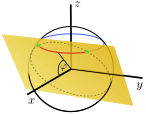
\includegraphics[width=0.6\linewidth]{circ_plane_intercept.pdf}
  \caption{Diagram showing the day-night plane (yellow) that passes through the
    origin at Earth's centre and rotates to face the sun, and the circle of
    constant latitude $\varphi$. The points where the circle intersects the plane
    (green) indicate the range of longitudes for which sunlight will reach Earth
  at latitude $\varphi$ (red) whilst longitudes on the opposite side of the
plane (blue) are in darkness.}
  \label{fig:circ_plane_intercept}
\end{figure}




Figure \ref{fig:daily_ave_insol_all_lats} shows
insolation across all latitudes during the year 2000. The Earth's orbital
parameters at this point are shown in Table \ref{tab:orbital_params}.


\begin{table}[h]
  \centering
  \caption{Earth's orbital parameters on the year 2000.}
\label{tab:orbital_params}
\begin{tabular}{lllll}
\multicolumn{1}{l|}{Eccentricity:} & 0.0167 &  &  &  \\ \cline{1-2}
\multicolumn{1}{l|}{Obliquity:}    & 0.4091 radians &  &  &  \\ \cline{1-2}
\multicolumn{1}{l|}{Precession:}   & 2.9161 radians &  &  &  \\
                                   &        &  &  &
\end{tabular}
\end{table}

\begin{figure}
  \centering
  \includegraphics[width=\linewidth]{both_daily_ave_insolation_all_lats.pdf}
  \caption{Contours showing the daily average insolation arriving at
    the atmosphere for different latitudes over a year period. The left plot is
  based on current orbital parameters, as shown in Table
\ref{tab:orbital_params}, the right plot is how the irradiance will be
distributed 1.015$\times10^6$ years from now, when eccentricity is 0.0582}
  \label{fig:daily_ave_insol_all_lats}
\end{figure}

\begin{figure}
  \centering
  \includegraphics[width=0.7\linewidth]{yearly_average_insol_150kN.pdf}
  \caption{Contour showing the difference in yearly average insolation from the
  average insolation over the 150k year period at each latitude. The lower
  plot shows how these fluctuations in yearly insolation correlate with Earth's
  obliquity.}
  \label{fig:yearly_ave_insol_all_lats}
\end{figure}

\begin{thebibliography}{30}
  \bibitem{milanko_data}
    Laskar J, Robutel P, Joutel F, Gastineau M, Correia AC, Levrard B. A
    long-term numerical solution for the insolation quantities of the Earth.
    Astronomy \& Astrophysics. 2004 Dec 1;428(1):261-85.
\end{thebibliography}
\end{document}
